\section{Diffusion equation}
\subsection{Diffusion equation derivation with Fourier's law}
Fourier's law for heat flow is
\begin{align} \label{eq:4.1}
	q = -k \grad{\theta}
\end{align}
where $q$ is the heat flux, $k$ the thermal conductivity and $\theta$ is the temperature.
In a volume $V$, the overall heat energy $Q$ is given by
\begin{align} \label{eq:4.2}
	Q = \int_V c_V \rho \theta \dd{V}
\end{align}
where $c_V$ is the specific heat of the material, $\rho$ is the mass density.
The rate of change due to heat flow is
\begin{align*}
	\dv{Q}{t} = \int_V c_V \rho \pdv{\theta}{t} \dd{V} \tag{$\ast$}
\end{align*}
We will integrate \cref{eq:4.1} over the surface $S = \partial V$, giving
\begin{align*}
	-\dv{Q}{t} = \int_S q \cdot \hat n \dd{S}
\end{align*}
The negative sign is due to the normals facing outwards.
This is exactly
\begin{align*}
	-\dv{Q}{t} = \int_S (-k \grad{\theta}) \cdot \hat n \dd{S} = \int_V -k \laplacian{\theta} \dd{V} \tag{$\dagger$}
\end{align*}
Equating these two forms (($\ast$) and ($\dagger$)) for $\dv{Q}{t}$, we find
\begin{align*}
	\int_V (c_V \rho \pdv{\theta}{t} - k \laplacian{\theta}) \dd{V} = 0
\end{align*}
Since $V$ was arbitrary, the integrand must be zero.
So we have
\begin{align*}
	\pdv{\theta}{t} - \frac{k}{c_V \rho} \laplacian{\theta} = 0
\end{align*}
Let $D = \frac{k}{c_V \rho}$ be the diffusion constant.
Then we have the diffusion equation
\begin{align} \label{eq:4.3}
	\pdv{\theta}{t} - D \laplacian{\theta} = 0
\end{align}

\subsection{Diffusion equation derivation with statistical dynamics}
We can derive this equation in another way, using statistical dynamics.
Gas particles diffuse by scattering every fixed time step $\Delta t$ with probability density function $p(\xi)$ of moving by a displacement $\xi$.
On average, we have
\begin{align*}
	\mathbb{E}[\xi] = \int p(\xi) \xi \dd{\xi} = 0
\end{align*}
since there is no bias the direction in which any given particle is travelling.
Suppose that the probability density function after $N\Delta t$ time is described by $P_{N \Delta t}(x)$.
Then, for the next time step,
\begin{align*}
	P_{(N+1)\Delta t}(x) = \int_{-\infty}^\infty p(\xi) P_{N \Delta t}(x - \xi) \dd{\xi}
\end{align*}
Using the Taylor expansion,
\begin{align*}
	P_{(N+1)\Delta t}(x) & \approx \int_{-\infty}^\infty p(\xi) \qty[P_{N \Delta t}(x) + P_{N \Delta t}'(x)(-\xi) + P_{N \Delta t}''(x)\frac{\xi^2}{2} + \cdots] \dd{\xi} \\
	& \approx P_{N \Delta t}(x) - P_{N \Delta t}'(x) \mathbb{E}[\xi] + P_{N \Delta t}''(x) \frac{\mathbb{E}[\xi^2]}{2} + \cdots \\
	& \approx P_{N \Delta t}(x) + P_{N \Delta t}''(x) \frac{\mathbb{E}[\xi^2]}{2} + \cdots
\end{align*}
since $\int p(\xi) \dd{\xi} = 1$.
Identifying $P_{N \Delta t}(x) = P(x, N\Delta t)$, we can write
\begin{align*}
	P(x, (N+1)\Delta t) - P(x, N \Delta t) = \pdv[2]{x} P(x, N\Delta t) \frac{\mathbb{E}[\xi^2]}{2}
\end{align*}
Assuming that the variance $\mathbb{E}[\xi^2]$\footnote{$\Var X = \mathbb{E}[X^2] - \mathbb{E}[X]^2$ and $\mathbb{E}[X] = 0$.} is equal to $2D \Delta t$, then for small $\Delta t$, we find
\begin{align} \label{eq:4.4}
	\pdv{P}{t} = D \pdv[2]{P}{x}
\end{align}
which is exactly the diffusion equation.

\subsection{Similarity solutions}
The characteristic relation between the variance and time suggests that we seek solutions with a dimensionless parameter.
If we can find a change of variables of the form $\theta(\eta) = \theta(x,t)$, then it will likely be easier to solve.
Consider
\begin{align} \label{eq:4.5}
	\eta \equiv \frac{x}{2\sqrt{Dt}}
\end{align}
Then changing variables in \cref{eq:4.3},
\begin{align*}
	\pdv{\theta}{t} = \pdv{\eta}{t} \pdv{\theta}{\eta} = \frac{-1}{2} \frac{x}{\sqrt{D} t^{3/2}} \theta' = \frac{-1}{2} \frac{\eta}{t} \theta'
\end{align*}
and
\begin{align*}
	D \pdv[2]{\theta}{x} = D \pdv{x} \qty(\pdv{\eta}{x} \pdv{\theta}{\eta}) = D \pdv{x} \qty(\frac{1}{2\sqrt{Dt}} \theta') = \frac{D}{4Dt} \theta'' = \frac{1}{4t} \theta''
\end{align*}
Equating,
\begin{align} \label{eq:4.6}
	\theta'' = -2 \eta \theta'
\end{align}
Let $\psi = \theta'$.
Then
\begin{align*}
	\frac{\psi'}{\psi} = -2\eta \implies \ln \psi = -\eta^2 + \text{constant}
\end{align*}
Then, choosing a constant of $c\frac{2}{\sqrt{\pi}}$,
\begin{align} \label{eq:4.7}
	\psi = c\frac{2}{\sqrt{\pi}} e^{-\eta^2} \implies \theta(\eta) = c\frac{2}{\sqrt{\pi}} \int_0^\eta e^{-u^2} \dd{u} = c \erf(\eta) = c \erf \qty(\frac{x}{2\sqrt{Dt}})
\end{align}
where
\begin{align*}
	\erf(z) = \frac{2}{\sqrt{\pi}} \int_0^z e^{-u^2} \dd{u}
\end{align*}
This describes discontinuous initial conditions that spread over time.

\begingroup
\tikzset{every picture/.style={scale=1}}
% Recommended preamble:
% \usetikzlibrary{arrows.meta}
% \usetikzlibrary{backgrounds}
% \usepgfplotslibrary{patchplots}
% \usepgfplotslibrary{fillbetween}
% \pgfplotsset{%
%     layers/standard/.define layer set={%
%         background,axis background,axis grid,axis ticks,axis lines,axis tick labels,pre main,main,axis descriptions,axis foreground%
%     }{
%         grid style={/pgfplots/on layer=axis grid},%
%         tick style={/pgfplots/on layer=axis ticks},%
%         axis line style={/pgfplots/on layer=axis lines},%
%         label style={/pgfplots/on layer=axis descriptions},%
%         legend style={/pgfplots/on layer=axis descriptions},%
%         title style={/pgfplots/on layer=axis descriptions},%
%         colorbar style={/pgfplots/on layer=axis descriptions},%
%         ticklabel style={/pgfplots/on layer=axis tick labels},%
%         axis background@ style={/pgfplots/on layer=axis background},%
%         3d box foreground style={/pgfplots/on layer=axis foreground},%
%     },
% }

\begin{tikzpicture}[/tikz/background rectangle/.style={fill={rgb,1:red,1.0;green,1.0;blue,1.0}, draw opacity={1.0}}, show background rectangle]
\begin{axis}[point meta max={nan}, point meta min={nan}, legend cell align={left}, legend columns={1}, title={$D=1$}, title style={at={{(0.5,1)}}, anchor={south}, font={{\fontsize{14 pt}{18.2 pt}\selectfont}}, color={rgb,1:red,0.0;green,0.0;blue,0.0}, draw opacity={1.0}, rotate={0.0}, align={center}}, legend style={color={rgb,1:red,0.0;green,0.0;blue,0.0}, draw opacity={1.0}, line width={1}, solid, fill={rgb,1:red,1.0;green,1.0;blue,1.0}, fill opacity={1.0}, text opacity={1.0}, font={{\fontsize{8 pt}{10.4 pt}\selectfont}}, text={rgb,1:red,0.0;green,0.0;blue,0.0}, cells={anchor={center}}, at={(1.02, 1)}, anchor={north west}}, axis background/.style={fill={rgb,1:red,1.0;green,1.0;blue,1.0}, opacity={1.0}}, anchor={north west}, xshift={1.0mm}, yshift={-1.0mm}, width={145.4mm}, height={99.6mm}, scaled x ticks={false}, xlabel={$x$}, x tick style={color={rgb,1:red,0.0;green,0.0;blue,0.0}, opacity={1.0}}, x tick label style={color={rgb,1:red,0.0;green,0.0;blue,0.0}, opacity={1.0}, rotate={0}}, xlabel style={at={(ticklabel cs:0.5)}, anchor=near ticklabel, at={{(ticklabel cs:0.5)}}, anchor={near ticklabel}, font={{\fontsize{11 pt}{14.3 pt}\selectfont}}, color={rgb,1:red,0.0;green,0.0;blue,0.0}, draw opacity={1.0}, rotate={0.0}}, xmajorgrids={true}, xmin={-3.18}, xmax={3.18}, xticklabels={{$-3$,$-2$,$-1$,$0$,$1$,$2$,$3$}}, xtick={{-3.0,-2.0,-1.0,0.0,1.0,2.0,3.0}}, xtick align={inside}, xticklabel style={font={{\fontsize{8 pt}{10.4 pt}\selectfont}}, color={rgb,1:red,0.0;green,0.0;blue,0.0}, draw opacity={1.0}, rotate={0.0}}, x grid style={color={rgb,1:red,0.0;green,0.0;blue,0.0}, draw opacity={0.1}, line width={0.5}, solid}, axis x line*={left}, x axis line style={color={rgb,1:red,0.0;green,0.0;blue,0.0}, draw opacity={1.0}, line width={1}, solid}, scaled y ticks={false}, ylabel={$\theta$}, y tick style={color={rgb,1:red,0.0;green,0.0;blue,0.0}, opacity={1.0}}, y tick label style={color={rgb,1:red,0.0;green,0.0;blue,0.0}, opacity={1.0}, rotate={0}}, ylabel style={at={(ticklabel cs:0.5)}, anchor=near ticklabel, at={{(ticklabel cs:0.5)}}, anchor={near ticklabel}, font={{\fontsize{11 pt}{14.3 pt}\selectfont}}, color={rgb,1:red,0.0;green,0.0;blue,0.0}, draw opacity={1.0}, rotate={0.0}}, ymajorgrids={true}, ymin={-1.06}, ymax={1.06}, yticklabels={{$-1.0$,$-0.5$,$0.0$,$0.5$,$1.0$}}, ytick={{-1.0,-0.5,0.0,0.5,1.0}}, ytick align={inside}, yticklabel style={font={{\fontsize{8 pt}{10.4 pt}\selectfont}}, color={rgb,1:red,0.0;green,0.0;blue,0.0}, draw opacity={1.0}, rotate={0.0}}, y grid style={color={rgb,1:red,0.0;green,0.0;blue,0.0}, draw opacity={0.1}, line width={0.5}, solid}, axis y line*={left}, y axis line style={color={rgb,1:red,0.0;green,0.0;blue,0.0}, draw opacity={1.0}, line width={1}, solid}, colorbar={false}]
    \addplot[color={rgb,1:red,0.0;green,0.6056;blue,0.9787}, name path={bbbde1b4-bfdc-4bb8-9cd6-47f3119a67c6}, draw opacity={1.0}, line width={1}, solid]
        table[row sep={\\}]
        {
            \\
            -3.0  -1.0  \\
            -2.9609367239208475  -1.0  \\
            -2.5997403313265086  -1.0  \\
            -2.3826763547775043  -1.0  \\
            -2.199151525136937  -1.0  \\
            -1.9997921198677944  -1.0  \\
            -1.8160003818614874  -1.0  \\
            -1.6189562143740408  -1.0  \\
            -1.3906612226458708  -1.0  \\
            -1.1877795755559142  -1.0  \\
            -1.00987065383912  -1.0  \\
            -0.8159021733787222  -1.0  \\
            -0.6207808849887516  -1.0  \\
            -0.5129151172455673  -1.0  \\
            -0.40504934950238297  -1.0  \\
            -0.30241779326150453  -1.0  \\
            -0.19978623702062615  -1.0  \\
            -0.14642973425411906  -1.0  \\
            -0.093073231487612  -1.0  \\
            -0.06639498010435846  -1.0  \\
            -0.03971672872110493  -1.0  \\
            -0.03304716587529155  -1.0  \\
            -0.026377603029478166  -1.0  \\
            -0.01970804018366478  -1.0  \\
            -0.0130384773378514  -1.0  \\
            -0.009703695914944709  -1.0  \\
            -0.006368914492038016  -1.0  \\
            -0.00470152378058467  -1.0  \\
            -0.003034133069131324  -1.0  \\
            -0.001366742357677978  -1.0  \\
            0.0003006483537753681  1.0  \\
            0.0019680390652287143  1.0  \\
            0.00363542977668206  1.0  \\
            0.005302820488135406  1.0  \\
            0.006970211199588752  1.0  \\
            0.010304992622495443  1.0  \\
            0.013639774045402136  1.0  \\
            0.02486847658427578  1.0  \\
            0.03609717912314943  1.0  \\
            0.047325881662023075  1.0  \\
            0.05855458420089672  1.0  \\
            0.08101198927864402  1.0  \\
            0.10346939435639131  1.0  \\
            0.1483842045118859  1.0  \\
            0.19329901466738048  1.0  \\
            0.41264258394545644  1.0  \\
            0.6135751697836116  1.0  \\
            0.7991519189555105  1.0  \\
            0.9871354150600441  1.0  \\
            1.1978122140406555  1.0  \\
            1.388719406219134  1.0  \\
            1.6072949743767582  1.0  \\
            1.8096765128752679  1.0  \\
            2.009200994923107  1.0  \\
            2.202922753671847  1.0  \\
            2.4015123274889874  1.0  \\
            2.6190902607646405  1.0  \\
            2.93515789239279  1.0  \\
            3.0  1.0  \\
        }
        ;
    \addlegendentry {$t=0$}
    \addplot[color={rgb,1:red,0.8889;green,0.4356;blue,0.2781}, name path={59314d39-cec7-4ae5-9cca-64005a7635a4}, draw opacity={1.0}, line width={1}, solid]
        table[row sep={\\}]
        {
            \\
            -3.0  -1.0  \\
            -2.9609367239208475  -1.0  \\
            -2.5997403313265086  -1.0  \\
            -2.3826763547775043  -1.0  \\
            -2.199151525136937  -1.0  \\
            -1.9997921198677944  -1.0  \\
            -1.8160003818614874  -1.0  \\
            -1.6189562143740408  -1.0  \\
            -1.3906612226458708  -1.0  \\
            -1.1877795755559142  -1.0  \\
            -1.00987065383912  -1.0  \\
            -0.8159021733787222  -1.0  \\
            -0.6207808849887516  -1.0  \\
            -0.5129151172455673  -1.0  \\
            -0.40504934950238297  -1.0  \\
            -0.3537335713819437  -0.9999999999999974  \\
            -0.30241779326150453  -0.9999999999864151  \\
            -0.25110201514106534  -0.9999999803223646  \\
            -0.19978623702062615  -0.9999920807742605  \\
            -0.17310798563737262  -0.9998915266778654  \\
            -0.14642973425411906  -0.9989406406086226  \\
            -0.1330906085624923  -0.9970796178516699  \\
            -0.11975148287086554  -0.992587585404849  \\
            -0.11308192002505216  -0.9885477823344052  \\
            -0.10641235717923878  -0.9826616292816677  \\
            -0.0997427943334254  -0.9742735736645938  \\
            -0.093073231487612  -0.9625826328591867  \\
            -0.0897384500647053  -0.9552090868523828  \\
            -0.0864036686417986  -0.9466460192128695  \\
            -0.08306888721889191  -0.9367566491563639  \\
            -0.07973410579598522  -0.9253988507524387  \\
            -0.07639932437307853  -0.9124268801068293  \\
            -0.07306454295017184  -0.8976934443929281  \\
            -0.06972976152726515  -0.8810521010229675  \\
            -0.06639498010435846  -0.8623599618888228  \\
            -0.06306019868145177  -0.8414806634259511  \\
            -0.05972541725854508  -0.8182875488181677  \\
            -0.056390635835638386  -0.7926669946093696  \\
            -0.053055854412731696  -0.7645218010252804  \\
            -0.049721072989825005  -0.7337745541652834  \\
            -0.046386291566918314  -0.7003708596205451  \\
            -0.04305151014401162  -0.6642823416736524  \\
            -0.03971672872110493  -0.6255093006010505  \\
            -0.03638194729819824  -0.5840829231549527  \\
            -0.03304716587529155  -0.5400669482891236  \\
            -0.02971238445238486  -0.49355870164745336  \\
            -0.026377603029478166  -0.4446894280627415  \\
            -0.02304282160657147  -0.39362387088969103  \\
            -0.01970804018366478  -0.3405590697701961  \\
            -0.01637325876075809  -0.2857223735481934  \\
            -0.0130384773378514  -0.22936869149833367  \\
            -0.006368914492038016  -0.11324640882870098  \\
            0.0003006483537753681  0.0053638993811737316  \\
            0.006970211199588752  0.12385556892554953  \\
            0.013639774045402136  0.23962974986643085  \\
            0.016446949680120546  0.286951512666272  \\
            0.019254125314838957  0.3331937279503094  \\
            0.02206130094955737  0.37820338860902075  \\
            0.02486847658427578  0.42184112721921957  \\
            0.027675652218994193  0.46398244623814067  \\
            0.030482827853712605  0.5045186807337945  \\
            0.033290003488431016  0.5433576837155185  \\
            0.03609717912314943  0.5804242308842567  \\
            0.03890435475786784  0.6156601482194205  \\
            0.04171153039258625  0.6490241720614864  \\
            0.044518706027304664  0.6804915570600641  \\
            0.047325881662023075  0.7100534523854313  \\
            0.05013305729674149  0.7377160708274008  \\
            0.0529402329314599  0.7634996787425251  \\
            0.05574740856617831  0.7874374372078601  \\
            0.05855458420089672  0.8095741261807469  \\
            0.061361759835615134  0.8299647839669007  \\
            0.06416893547033355  0.8486732939118713  \\
            0.06697611110505196  0.8657709490289307  \\
            0.06978328673977037  0.8813350233570115  \\
            0.07259046237448878  0.8954473763196841  \\
            0.0753976380092072  0.9081931133556759  \\
            0.0782048136439256  0.9196593227441014  \\
            0.08101198927864402  0.9299339049845103  \\
            0.08662634054808084  0.9472575733238839  \\
            0.09224069181751766  0.9608459833298386  \\
            0.09785504308695449  0.9713380658048624  \\
            0.10346939435639131  0.9793128514223746  \\
            0.10908374562582812  0.9852796393459977  \\
            0.11469809689526494  0.9896743111476254  \\
            0.12031244816470177  0.9928605369310586  \\
            0.1259267994341386  0.9951345392296561  \\
            0.13715550197301224  0.9978370174858159  \\
            0.1483842045118859  0.9990932632288029  \\
            0.17084160958963318  0.9998666210921499  \\
            0.19329901466738048  0.9999845587122477  \\
            0.24813490698689947  0.9999999711811763  \\
            0.30297079930641846  0.9999999999875278  \\
            0.3578066916259375  0.9999999999999988  \\
            0.41264258394545644  1.0  \\
            0.513108876864534  1.0  \\
            0.6135751697836116  1.0  \\
            0.7991519189555105  1.0  \\
            0.9871354150600441  1.0  \\
            1.1978122140406555  1.0  \\
            1.388719406219134  1.0  \\
            1.6072949743767582  1.0  \\
            1.8096765128752679  1.0  \\
            2.009200994923107  1.0  \\
            2.202922753671847  1.0  \\
            2.4015123274889874  1.0  \\
            2.6190902607646405  1.0  \\
            2.93515789239279  1.0  \\
            3.0  1.0  \\
        }
        ;
    \addlegendentry {$t = 10^{-3}$}
    \addplot[color={rgb,1:red,0.2422;green,0.6433;blue,0.3044}, name path={6232a22f-da1a-4c5f-bc6f-625fd2918cd1}, draw opacity={1.0}, line width={1}, solid]
        table[row sep={\\}]
        {
            \\
            -3.0  -1.0  \\
            -2.9609367239208475  -1.0  \\
            -2.5997403313265086  -1.0  \\
            -2.3826763547775043  -1.0  \\
            -2.199151525136937  -1.0  \\
            -1.9997921198677944  -1.0  \\
            -1.8160003818614874  -1.0  \\
            -1.6189562143740408  -1.0  \\
            -1.3906612226458708  -1.0  \\
            -1.1877795755559142  -1.0  \\
            -1.00987065383912  -0.9999999999990725  \\
            -0.8159021733787222  -0.9999999920398323  \\
            -0.6207808849887516  -0.999988643215685  \\
            -0.5668480011171595  -0.9999388220531092  \\
            -0.5129151172455673  -0.9997131085680446  \\
            -0.45898223337397515  -0.9988275316927056  \\
            -0.40504934950238297  -0.9958184551343818  \\
            -0.3793914604421633  -0.9926970129518808  \\
            -0.3537335713819437  -0.9876252628633458  \\
            -0.3280756823217241  -0.9796507577343972  \\
            -0.30241779326150453  -0.9675170636513158  \\
            -0.28958884873139473  -0.9594108301709481  \\
            -0.27675990420128493  -0.9496511266833726  \\
            -0.26393095967117514  -0.9379969194652074  \\
            -0.25110201514106534  -0.9241944293155557  \\
            -0.23827307061095554  -0.9079815274514302  \\
            -0.22544412608084574  -0.8890932366540245  \\
            -0.21261518155073594  -0.8672682912771007  \\
            -0.19978623702062615  -0.8422566454994204  \\
            -0.18644711132899938  -0.8126235835725499  \\
            -0.17310798563737262  -0.7790697666197243  \\
            -0.15976885994574586  -0.7414127036366686  \\
            -0.14642973425411906  -0.6995246606893336  \\
            -0.1330906085624923  -0.6533426531858829  \\
            -0.11975148287086554  -0.6028771442900945  \\
            -0.10641235717923878  -0.5482189073424177  \\
            -0.093073231487612  -0.4895435567034366  \\
            -0.07973410579598522  -0.4271133344608578  \\
            -0.06639498010435846  -0.36127585721187666  \\
            -0.053055854412731696  -0.2924596718988572  \\
            -0.03971672872110493  -0.22116663394829106  \\
            -0.0130384773378514  -0.07345765012125084  \\
            0.013639774045402136  0.07683504383068354  \\
            0.03609717912314943  0.20146658764768505  \\
            0.05855458420089672  0.3211577031628891  \\
            0.06978328673977037  0.37829993705741255  \\
            0.08101198927864402  0.43324782699217496  \\
            0.09224069181751766  0.48575376102908213  \\
            0.10346939435639131  0.5356111259612224  \\
            0.11469809689526494  0.582656163336171  \\
            0.1259267994341386  0.6267686843337225  \\
            0.13715550197301224  0.6678716825237805  \\
            0.1483842045118859  0.7059299215437114  \\
            0.15961290705075953  0.7409476072284354  \\
            0.17084160958963318  0.7729652794710861  \\
            0.18207031212850683  0.8020560773038202  \\
            0.19329901466738048  0.8283215410471984  \\
            0.20700798774726023  0.8567425199211242  \\
            0.22071696082713999  0.8814065339278863  \\
            0.2344259339070197  0.9026101874489814  \\
            0.24813490698689947  0.9206686117630558  \\
            0.2618438800667792  0.935904620771657  \\
            0.27555285314665895  0.9486392058987063  \\
            0.28926182622653873  0.9591835748376183  \\
            0.30297079930641846  0.9678328277587064  \\
            0.33038874546617797  0.980519243423162  \\
            0.3578066916259375  0.9885961976222444  \\
            0.38522463778569693  0.9935493638073194  \\
            0.41264258394545644  0.9964751641207977  \\
            0.4628757304049952  0.9989359718937953  \\
            0.513108876864534  0.9997146264359955  \\
            0.5633420233240728  0.999932072213213  \\
            0.6135751697836116  0.9999856627398552  \\
            0.7991519189555105  0.9999999840350515  \\
            0.9871354150600441  0.9999999999970504  \\
            1.1978122140406555  1.0  \\
            1.388719406219134  1.0  \\
            1.6072949743767582  1.0  \\
            1.8096765128752679  1.0  \\
            2.009200994923107  1.0  \\
            2.202922753671847  1.0  \\
            2.4015123274889874  1.0  \\
            2.6190902607646405  1.0  \\
            2.93515789239279  1.0  \\
            3.0  1.0  \\
        }
        ;
    \addlegendentry {$t = 10^{-2}$}
    \addplot[color={rgb,1:red,0.7644;green,0.4441;blue,0.8243}, name path={5b059462-f580-4bc3-927d-d091966c8ddf}, draw opacity={1.0}, line width={1}, solid]
        table[row sep={\\}]
        {
            \\
            -3.0  -0.9999999999802965  \\
            -2.9609367239208475  -0.9999999999642875  \\
            -2.5997403313265086  -0.9999999938708811  \\
            -2.3826763547775043  -0.9999999006048895  \\
            -2.199151525136937  -0.9999991232218955  \\
            -1.9997921198677944  -0.9999922389279503  \\
            -1.8160003818614874  -0.9999510742576445  \\
            -1.6189562143740408  -0.9997055064352888  \\
            -1.3906612226458708  -0.9981266740459626  \\
            -1.2892203991008926  -0.996058229330461  \\
            -1.1877795755559142  -0.9920916038051636  \\
            -1.098825114697517  -0.98599158960537  \\
            -1.00987065383912  -0.9760630319759493  \\
            -0.9613785337240206  -0.9684216612329685  \\
            -0.9128864136089211  -0.9587766063969309  \\
            -0.8643942934938216  -0.9467446310665077  \\
            -0.8159021733787222  -0.9319102999877525  \\
            -0.7671218512812296  -0.9137164692541145  \\
            -0.718341529183737  -0.8917833125426629  \\
            -0.6695612070862442  -0.8656547099010363  \\
            -0.6207808849887516  -0.8348959176479536  \\
            -0.5938144430529555  -0.815758939248996  \\
            -0.5668480011171595  -0.7950272468173949  \\
            -0.5398815591813634  -0.7726494382101249  \\
            -0.5129151172455673  -0.7485824491553721  \\
            -0.4859486753097712  -0.7227926848408014  \\
            -0.45898223337397515  -0.6952570943935861  \\
            -0.43201579143817903  -0.6659641638905588  \\
            -0.40504934950238297  -0.6349148036285647  \\
            -0.3793914604421633  -0.6037541899450509  \\
            -0.3537335713819437  -0.5710398508393102  \\
            -0.3280756823217241  -0.5368071509610597  \\
            -0.30241779326150453  -0.5011033044668204  \\
            -0.27675990420128493  -0.4639874286318324  \\
            -0.25110201514106534  -0.42553044013826347  \\
            -0.22544412608084574  -0.3858147892936949  \\
            -0.19978623702062615  -0.3449340304976142  \\
            -0.14642973425411906  -0.25665493091768976  \\
            -0.093073231487612  -0.1648632237043389  \\
            -0.03971672872110493  -0.0707665376161081  \\
            0.013639774045402136  0.02433127752607976  \\
            0.05855458420089672  0.10417092401891336  \\
            0.10346939435639131  0.18296843529616683  \\
            0.1483842045118859  0.25995757718556245  \\
            0.19329901466738048  0.33442555133647794  \\
            0.22071696082713999  0.3783675939685244  \\
            0.24813490698689947  0.42100035518126816  \\
            0.27555285314665895  0.46220771620717255  \\
            0.30297079930641846  0.5018879538003761  \\
            0.33038874546617797  0.5399543571937845  \\
            0.3578066916259375  0.5763356014049799  \\
            0.38522463778569693  0.6109758794934395  \\
            0.41264258394545644  0.6438348015677368  \\
            0.43775915717522584  0.6723504624507537  \\
            0.4628757304049952  0.6993411753293457  \\
            0.4879923036347646  0.7248080571352101  \\
            0.513108876864534  0.7487614861836827  \\
            0.5382254500943033  0.7712204708068556  \\
            0.5633420233240728  0.7922119501280058  \\
            0.5884585965538423  0.8117700417603212  \\
            0.6135751697836116  0.8299352512613053  \\
            0.6599693570765863  0.8599853151462249  \\
            0.7063635443695611  0.8857732895562674  \\
            0.7527577316625358  0.9076669977091159  \\
            0.7991519189555105  0.9260557253674235  \\
            0.8461477929816439  0.9415148792772384  \\
            0.8931436670077773  0.9541889321493429  \\
            0.9401395410339106  0.9644656343181565  \\
            0.9871354150600441  0.9727070247171536  \\
            1.039804614805197  0.9799319857760929  \\
            1.0924738145503499  0.9854280345188169  \\
            1.1451430142955026  0.9895513713318527  \\
            1.1978122140406555  0.9926022870830888  \\
            1.2932658101298946  0.9961699519476673  \\
            1.388719406219134  0.9980989523433339  \\
            1.6072949743767582  0.9996743862024866  \\
            1.8096765128752679  0.9999480241265823  \\
            2.009200994923107  0.9999929677484587  \\
            2.202922753671847  0.999999160206309  \\
            2.4015123274889874  0.9999999212392595  \\
            2.6190902607646405  0.9999999952717359  \\
            2.93515789239279  0.9999999999473393  \\
            3.0  0.9999999999802965  \\
        }
        ;
    \addlegendentry {$t = 10^{-1}$}
    \addplot[color={rgb,1:red,0.6755;green,0.5557;blue,0.0942}, name path={0cf45548-f4cb-4113-812c-0099f95a8aac}, draw opacity={1.0}, line width={1}, solid]
        table[row sep={\\}]
        {
            \\
            -3.0  -0.9661051464753108  \\
            -2.9804683619604235  -0.9649265513695182  \\
            -2.9609367239208475  -0.9637131476610028  \\
            -2.780338527623678  -0.9507009535411899  \\
            -2.5997403313265086  -0.9339809078317416  \\
            -2.4912083430520067  -0.9218546947755499  \\
            -2.3826763547775043  -0.9079741103736406  \\
            -2.2909139399572207  -0.8947507050232054  \\
            -2.199151525136937  -0.8800622557069969  \\
            -2.0994718225023656  -0.8623371333225704  \\
            -1.9997921198677944  -0.8426576421642085  \\
            -1.9078962508646409  -0.8226907765011833  \\
            -1.8160003818614874  -0.800895195630151  \\
            -1.717478298117764  -0.7754204617158442  \\
            -1.6189562143740408  -0.7476975919364297  \\
            -1.5048087185099557  -0.7126986837363251  \\
            -1.3906612226458708  -0.6745628129799148  \\
            -1.2892203991008926  -0.6380293595393353  \\
            -1.1877795755559142  -0.5990282485263874  \\
            -1.098825114697517  -0.5628333768753401  \\
            -1.00987065383912  -0.5248262371810903  \\
            -0.9128864136089211  -0.4814020767489276  \\
            -0.8159021733787222  -0.4360132290296584  \\
            -0.718341529183737  -0.3885075003436815  \\
            -0.6207808849887516  -0.33930830126002426  \\
            -0.40504934950238297  -0.22543828953726075  \\
            -0.19978623702062615  -0.11234351191459552  \\
            0.013639774045402136  0.007695299133184976  \\
            0.19329901466738048  0.10871866739332182  \\
            0.41264258394545644  0.22954697379827776  \\
            0.6135751697836116  0.3356121891295767  \\
            0.7063635443695611  0.3825548196293288  \\
            0.7991519189555105  0.42798455343073566  \\
            0.8931436670077773  0.47231768843832095  \\
            0.9871354150600441  0.5148291509948483  \\
            1.0924738145503499  0.560179073273832  \\
            1.1978122140406555  0.6029943656709459  \\
            1.2932658101298946  0.6395337547604393  \\
            1.388719406219134  0.6738868053395398  \\
            1.4980071902979462  0.7105145352535559  \\
            1.6072949743767582  0.7442648378289973  \\
            1.708485743626013  0.7729842215155165  \\
            1.8096765128752679  0.7993263015146979  \\
            1.9094387538991873  0.823040815268532  \\
            2.009200994923107  0.8446017218668409  \\
            2.106061874297477  0.8635680882796628  \\
            2.202922753671847  0.8806960031086348  \\
            2.3022175405804175  0.896456800101484  \\
            2.4015123274889874  0.9105159509688344  \\
            2.5103012941268137  0.924110544584302  \\
            2.6190902607646405  0.9359708001764229  \\
            2.7771240765787155  0.9504378071140105  \\
            2.93515789239279  0.9620570081267613  \\
            2.967578946196395  0.9641297507378738  \\
            3.0  0.9661051464753108  \\
        }
        ;
    \addlegendentry {$t = 10^{0}$}
    \addplot[color={rgb,1:red,0.0;green,0.6658;blue,0.681}, name path={6c348c63-e572-40ab-ad16-8281c07017b0}, draw opacity={1.0}, line width={1}, solid]
        table[row sep={\\}]
        {
            \\
            -3.0  -0.4976650456394979  \\
            -2.9609367239208475  -0.4920836227218486  \\
            -2.5997403313265086  -0.43897493384921343  \\
            -2.3826763547775043  -0.40581594060647647  \\
            -2.199151525136937  -0.377100540780792  \\
            -1.9997921198677944  -0.3452455946644038  \\
            -1.8160003818614874  -0.3153088542753728  \\
            -1.6189562143740408  -0.28265515450352807  \\
            -1.3906612226458708  -0.24416995989970192  \\
            -1.1877795755559142  -0.20944931561484767  \\
            -1.00987065383912  -0.1786538678263862  \\
            -0.8159021733787222  -0.1447635613129309  \\
            -0.6207808849887516  -0.11040036093870902  \\
            -0.40504934950238297  -0.07216715029243596  \\
            -0.19978623702062615  -0.03563249183921455  \\
            0.013639774045402136  0.0024335012085193544  \\
            0.19329901466738048  0.0344762081473073  \\
            0.41264258394545644  0.07351622797628538  \\
            0.6135751697836116  0.10912695624295243  \\
            0.7991519189555105  0.14182343396963817  \\
            0.9871354150600441  0.17469747633775828  \\
            1.1978122140406555  0.21117671475710043  \\
            1.388719406219134  0.24383984504426923  \\
            1.6072949743767582  0.2807056827678866  \\
            1.8096765128752679  0.3142695889326951  \\
            2.009200994923107  0.3467638252990227  \\
            2.202922753671847  0.3776966264962377  \\
            2.4015123274889874  0.4087285738978299  \\
            2.6190902607646405  0.4418868302827166  \\
            2.93515789239279  0.4883825569441998  \\
            3.0  0.4976650456394979  \\
        }
        ;
    \addlegendentry {$t = 10^{1}$}
    \addplot[color={rgb,1:red,0.9308;green,0.3675;blue,0.5758}, name path={2c2c61b2-98fc-4354-97c6-10de65e7707e}, draw opacity={1.0}, line width={1}, solid]
        table[row sep={\\}]
        {
            \\
            -3.0  -0.1679959714273635  \\
            -2.9609367239208475  -0.16584046763179164  \\
            -2.5997403313265086  -0.14585271008390657  \\
            -2.3826763547775043  -0.13379484334786584  \\
            -2.199151525136937  -0.123575601648419  \\
            -1.9997921198677944  -0.11245130432503045  \\
            -1.8160003818614874  -0.1021759715938047  \\
            -1.6189562143740408  -0.09114071194101031  \\
            -1.3906612226458708  -0.07833339399770965  \\
            -1.1877795755559142  -0.06693458328127802  \\
            -1.00987065383912  -0.05692746556093605  \\
            -0.8159021733787222  -0.04600682717913549  \\
            -0.6207808849887516  -0.03501256657461558  \\
            -0.40504934950238297  -0.022849338358386186  \\
            -0.19978623702062615  -0.011271356475898262  \\
            0.013639774045402136  0.0007695417245292686  \\
            0.19329901466738048  0.010905389495376918  \\
            0.41264258394545644  0.02327756174444435  \\
            0.6135751697836116  0.034606414584226204  \\
            0.7991519189555105  0.04506333471034082  \\
            0.9871354150600441  0.05564796037962812  \\
            1.1978122140406555  0.06749860454013834  \\
            1.388719406219134  0.07822436640636275  \\
            1.6072949743767582  0.09048706307760562  \\
            1.8096765128752679  0.10182210482641191  \\
            2.009200994923107  0.11297683765183363  \\
            2.202922753671847  0.12378580904553153  \\
            2.4015123274889874  0.1348424551375436  \\
            2.6190902607646405  0.14692598650013727  \\
            2.93515789239279  0.16441731290492673  \\
            3.0  0.1679959714273635  \\
        }
        ;
    \addlegendentry {$t = 10^{2}$}
\end{axis}
\end{tikzpicture}

\endgroup

\subsection{Heat conduction in a finite bar}
Suppose we have a bar of length $2L$ with $-L \leq x \leq L$ and initial temperature
\begin{align} \label{eq:4.8}
	\theta(x,0) = H(x) = \begin{cases}
		1 & \text{if } 0 \leq x \leq L \\
		0 & \text{if } -L \leq x < 0
	\end{cases}
\end{align}
with boundary conditions
\begin{align} \label{eq:4.9}
    \theta(L, t) = 1, \quad \theta(-L, t) = 0.
\end{align}

\subsubsection{Transforming boundary conditions}
Currently the boundary conditions \cref{eq:4.9} are not homogeneous, so Sturm-Liouville theory cannot be used directly.
If we can identify a steady-state solution (time-independent) that reflects the late-time behaviour, then we can turn it into a homogeneous set of boundary conditions.
We will try a solution of the form
\begin{align*}
	\theta_s(x) = Ax + B
\end{align*}
since this certainly satisfies the diffusion equation.
To satisfy the boundary conditions \cref{eq:4.9},
\begin{align*}
	A = \frac{1}{2L};\quad B = \frac{1}{2}
\end{align*}
Hence we have a solution
\begin{align} \label{eq:4.10}
	\theta_s = \frac{x + L}{2L}
\end{align}
We will subtract this solution from our original equation for $\theta$, giving
\begin{align*}
	\hat \theta(x,t) = \theta(x,t) - \theta_s(x)
\end{align*}
with homogeneous boundary conditions
\begin{align*}
	\hat \theta(-L, t) = \hat \theta(L, t) = 0
\end{align*}
and initial conditions
\begin{align} \label{eq:4.11}
	\hat \theta(x,0) = H(x) - \frac{x+L}{2L}
\end{align}

\begin{figure}[h]
    \centering
    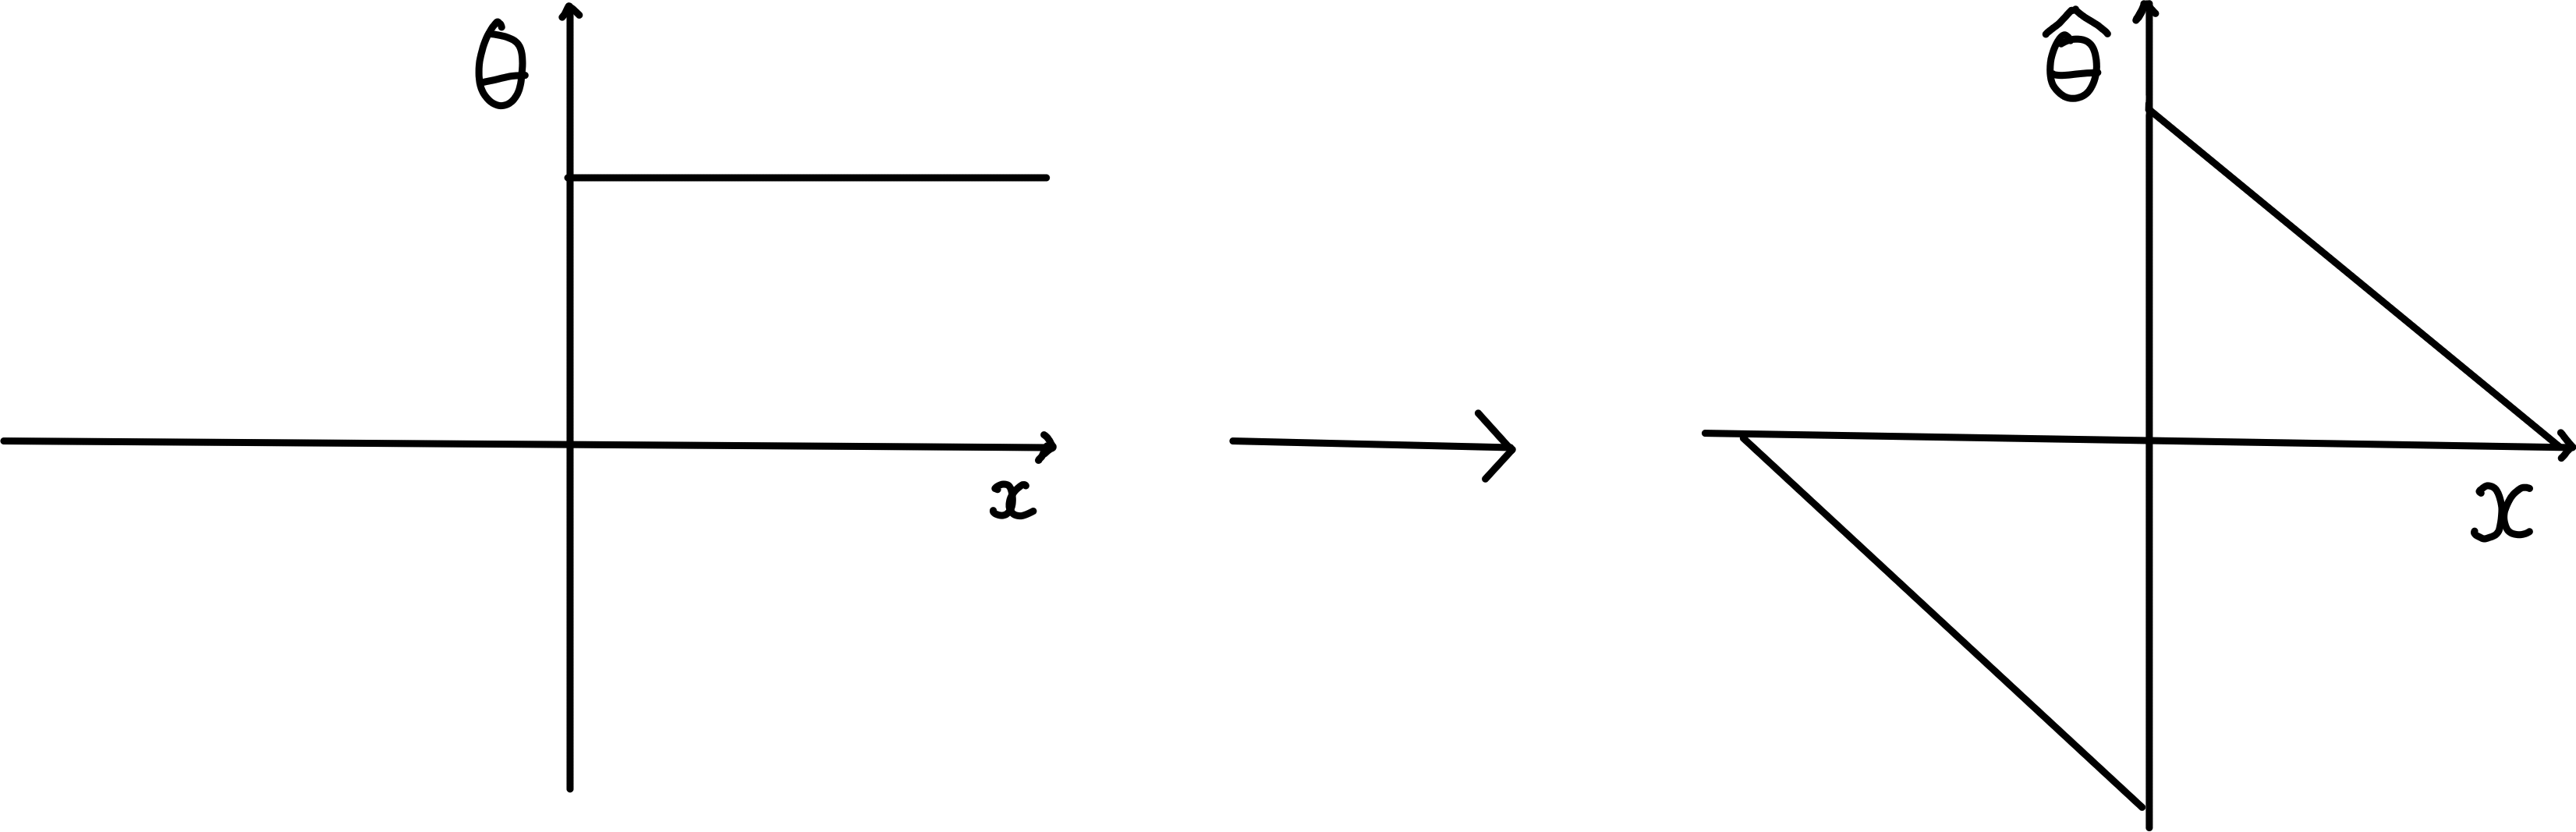
\includegraphics[height=5cm]{04-transformbcs}
\end{figure}

\subsubsection{Seperation of variables}
We will now separate variables in the usual way.
We will consider the ansatz
\begin{align} \label{eq:4.12}
	\hat \theta(x,t) = X(x) T(t) \implies X'' = - \lambda X; \dot T = -D \lambda T
\end{align}
The boundary conditions imply $\lambda > 0$ and give the Fourier modes $X(x) = A \cos \sqrt{\lambda} x + B \sin \sqrt{\lambda} x$.
For $\cos \sqrt{\lambda} L = 0$, we require $\sqrt{\lambda_m} = \frac{m \pi}{2L}$ for $m$ odd.
Also, $\sin \sqrt{\lambda} L = 0$ gives $\sqrt{\lambda_n} = \frac{n \pi}{L}$ for $n$ even.
Since $\hat \theta$ is odd due to our initial conditions, we can take
\begin{align*}
	X_n = B_n \sin \frac{n \pi x}{L}; \quad \lambda_n = \frac{n^2 \pi^2}{L^2}
\end{align*}
Substituting $\lambda_n$ into \cref{eq:4.12}, $\dot T = -D \lambda T$, we have
\begin{align*}
	T_n(t) = C_n \exp(-\frac{Dn^2 \pi^2}{L^2} t ).
\end{align*}
In general, the solution is
\begin{align} \label{eq:4.13}
	\hat \theta(x,t) = \sum_{n=1}^\infty b_n \sin \frac{n \pi x}{L} \exp(-\frac{Dn^2 \pi^2}{L^2} t )
\end{align}

\subsection{Particular solution to diffusion equation}
At $t = 0$, we have a pure Fourier sine series.
We can then impose the initial conditions \cref{eq:4.11}, to give
\begin{align*}
	b_n = \frac{1}{L} \int_{-L}^L \hat \phi(x,0) \sin \frac{n \pi x}{L} \dd{x}
\end{align*}
where
\begin{align*}
	\hat\phi(x,0) = H(x) - \frac{x+L}{2L}
\end{align*}
Hence, we can use the half-range sine series and find
\begin{align*}
	b_n = \underbrace{ \frac{2}{L} \int_0^L \qty(H(x) - \frac{1}{2}) \sin \frac{n \pi x}{L} \dd{x} }_{\text{square wave}/2, \ \cref{eq:1.7}} - \underbrace{ \frac{2}{L} \int_0^L \frac{x}{2L} \sin \frac{n \pi x}{L} \dd{x} }_{\text{sawtooth}/2L, \ \cref{eq:1.6}}
\end{align*}
which gives
\begin{align*}
	b_n = \frac{2}{(2m-1)\pi} - \frac{(-1)^{n+1}}{n\pi}
\end{align*}
where $n = 2m - 1$, and the first term vanishes for $n$ even.
For $n$ odd or even, we find the same result
\begin{align*}
	b_n = \frac{1}{n\pi}
\end{align*}
Hence
\begin{align*}
	\hat\theta(x,t) = \sum_{n=1}^\infty \frac{1}{n \pi} \sin \frac{n \pi x}{L} \exp\qty(-D \frac{n^2 \pi^2}{L^2} t)
\end{align*}
For the inhomogeneous boundary conditions,
\begin{align} \label{eq:4.14}
	\theta(x,t) = \frac{x+L}{2L} + \hat\theta(x,t)
\end{align}
The similarity solution $\frac{1}{2}\qty(1 + \erf(\frac{x}{2\sqrt{Dt}}))$, \cref{eq:4.7}, is a good fit for early $t$ (excellent for $t \leq 1$), but it does not necessarily satisfy the boundary conditions, so for large $t$ it is a bad approximation.

Plot with $L = 1$ and $D = 1$
insertpicture